\documentclass[handout, notes=hide]{beamer}

\usepackage{attrib}
\graphicspath{{./figures/}}
\DeclareGraphicsExtensions{.pdf,.jpeg,.png,.jpg}
\usepackage[export]{adjustbox}

\usetheme{Rochester}
\usecolortheme{beaver}

\setbeamertemplate{bibliography entry title}{}
\setbeamertemplate{bibliography entry location}{}
\setbeamertemplate{bibliography entry note}{}

\renewcommand{\thefootnote}{\fnsymbol{footnote}}
\newcommand{\prescite}[1]{\footnote{\cite{#1}}}
\usepackage{perpage}
\MakePerPage{footnote}

\begin{document}

\title{Information Security: Where Computer Science, Economics and Psychology Meet}
\subtitle{R209, Paper by Ross Anderson and Tyler Moore, 2009}
\author{David Llewellyn-Jones}
\institute{
\href{mailto:dl551@cam.ac.uk}{dl551@cam.ac.uk}\\
Computer Laboratory\\
University of Cambridge}
\date{2nd November 2015}

%%%%%%%%%%%%%%%%%%%%%%%%%%%%%%%%%%%%%%%%%

\frame{\titlepage}

%%%%%%%%%%%%%%%%%%%%%%%%%%%%%%%%%%%%%%%%%

\begin{frame}

\frametitle{Information Security}
\framesubtitle{Where Computer Science, Economics and Psychology Meet}
\begin{columns}[b]
\begin{column}[c]{0.5\textwidth}
\setlength{\parskip}{0.5em}

Survey of topics broadening the scope of information security.

A manifesto for multidisciplinarity in information security.

Developed from keynote at 18th Symposium on Operating Systems Principles, 2001, ``Why Information Security is Hard -- An Economic Perspective''.
\end{column}
\begin{column}[c]{0.48\textwidth}
\includegraphics[width=\textwidth, frame]{paperfront}
\end{column}
\end{columns}
\end{frame}

%%%%%%%%%%%%%%%%%%%%%%%%%%%%%%%%%%%%%%%%%

\begin{frame}

\frametitle{Information Security}
\framesubtitle{Where Computer Science, Economics and Psychology Meet}
Grew from a failure of traditional information security techniques.

\begin{quote}
``According to one common view, information security comes down to technical measures... I put forward a contrary view: information insecurity is at least as much due to perverse incentives.''
\attrib{Ross Anderson, 2001\prescite{anderson2001}}
\end{quote}

\note{Compare to Karger and Schell: ``Multics can be developed into an open secure multi-level system by restructuring the operating system to include a security kernel.''.\\
Some key dates:
{\tiny
\begin{enumerate}
\item 1999: Bruce Schneier, ``Attack Trees'', Dr. Dobb's.
\item 2001: Ross Anderson, ``Why Information Security is Hard -- An Economic Perspective'', ACSAC 2001.
\item 2002: Bill Gate's ``Trustworthy Computing'' internal memo.
\item 2008: Ross Anderson, Rainer Boehme, Richard Clayton, Tyler Moore, ``Security Economics and the Internal Market -- ENISA'', ENISA report.
\item 2009: Ross Anderson, Tyler Moore, ``Information security: where computer science, economics and psychology meet'', Philosophical Transactions of the Royal Society of London A: Mathematical, Physical and Engineering Sciences.
\item 2011: Detica, ``The Cost of Cyber Crime'', Cabinet Office: \pounds 3.1bn (citizens), \pounds 2.22bn (government), \pounds 21bn (businesses).
\item 2012: Anderson {\it etal.}, ``Measuring the Cost of Cybercrime'', The Economics of Information Security and Privacy, Springer.
\end{enumerate}
}
}%
\end{frame}

%%%%%%%%%%%%%%%%%%%%%%%%%%%%%%%%%%%%%%%%%

\begin{frame}
\frametitle{Aims}
\setlength{\parskip}{0.5em}

\begin{quote}
``Why is it... that most people care too little about online security and privacy, yet overreact to terrorism?''
\end{quote}

Initial paper focusses on misaligned incentives. The 2009 paper presents a more holistic view.

Reviews recent results and live research challenges in the area.

\begin{enumerate}
\item Study of the impact of externalities.
\item Asymmetric information.
\item Application of the ideas from the boundary between economics and psychology.
\end{enumerate}

\end{frame}

%%%%%%%%%%%%%%%%%%%%%%%%%%%%%%%%%%%%%%%%%

\begin{frame}
\frametitle{Themes}

Highlights six themes.
\begin{enumerate}
\item Misaligned incentives.
\item Security as an externality.
\item Economics of vulnerabilities.
\item Economics of privacy.
\item Social networks and information security.
\item Psychology.
\end{enumerate}

\end{frame}

%%%%%%%%%%%%%%%%%%%%%%%%%%%%%%%%%%%%%%%%%

\begin{frame}
\frametitle{Misaligned Incentives}
\setlength{\parskip}{0.5em}

Grew from an observation about banking fraud in the early nineties\prescite{anderson1994}.

\begin{enumerate}
\item US banks more liable for cost of card fraud than UK banks.
\item UK bank staff became lazy and careless.
\item Led to an avalanche of fraud.
\item Decreased liability led to increased spend on security \& fraud.
\end{enumerate}
Takeaway: ``Liability should be assigned to whoever can best manage the risk.''

Example of a {\it moral hazard effect}\prescite{dembe2000}.

\end{frame}
\note{
``the tendency for insurance plans to encourage behavior that increases the risk of insured loss.''\\
Quote from Dembe and Boden, ``Moral Hazard: A Question of Morality'', 2000.\\
When one party takes on risk because another party takes on the burden of those risks.\\
The insured party takes on the risk because the insurer is taking on the burden of those risks.
}
%%%%%%%%%%%%%%%%%%%%%%%%%%%%%%%%%%%%%%%%%

\begin{frame}
\frametitle{Asymmetric Information}

Akerlof identified this as resulting from {\it asymmetric information}\prescite{akerlof1970}.

\begin{enumerate}
\item Town with 50 good cars and 50 `lemons'.
\item Good cars worth \$2000, lemons worth \$1000.
\item Sellers can tell difference, buyers can't.
\item From buyers' perspective, will buy cars for \$1500.
\item But sellers of good cars won't sell at this price.
\item Market deteriorates to that of the lemons.
\end{enumerate}

\end{frame}
\note{
G. A. Akerlof, ``The market for lemons: Quality uncertainty and the market mechanism,'' The
Quarterly Journal of Economics, 84(3):488–500, 1970.\\
Software is a market with asymmetric information.\\
Buyers can't tell the difference between secure and insecure software.\\  
Can extend `hidden information' to `hidden action'.\\
Also arises in protocols such as P2P filesharing or TCP backoff algorithm.}

%%%%%%%%%%%%%%%%%%%%%%%%%%%%%%%%%%%%%%%%%

\begin{frame}
\frametitle{Externalities}

An {\it externality\/} is present when
$$
u^A = u^A(X_1, X_2, \ldots, X_m, Y_1).
$$
The utility of an individual $A$ is dependent on the `activities' $(X_1, \ldots, X_m)$ that are exclusively under her control, but also upon another single activity $Y_1$ under the control of $B$\prescite{buchanan1962}.

\end{frame}
\note{
J. M. Buchanan, W. C. Stubblebine, ``Externality,'' Economica, 29(116):371–384, 1962.\\
$B$ is presumed to be a member of the same social group as $A$.\\
Buchanan and Stubblebine partition this further into {\it marginal externalities}, {\it infra-marginal externalities}, {\it economies}, {\it diseconomies}, {\it relevant externalities}, {\it irrelevant externalities\/} and {\it Pareto-relevant marginal externalities}.\\
Edgeworth box diagram.}

%%%%%%%%%%%%%%%%%%%%%%%%%%%%%%%%%%%%%%%%%

\begin{frame}
\frametitle{Externalities}
\framesubtitle{Buchanan and Stubblebine's improbable fence}
\begin{columns}[T]
\begin{column}[T]{0.5\textwidth}
\includegraphics[width=\textwidth]{fence-actors}
\end{column}
\begin{column}[T]{0.5\textwidth}
\includegraphics[width=\textwidth]{fence-graphnolines}
\end{column}
\end{columns}

\end{frame}
\note{
{\footnotesize Consider two persons, $A$ and $B$, who own adjoining units of residential property. Within limits to be noted, each person values privacy, which may be measured quantitatively in terms of a single criterion, the height of a fence that can be constructed along the common boundary line. We shall assume that $B$'s desire for privacy holds over rather wide limits. His utility increases with the height of the fence up to a reasonably high level. Up to a certain minimum height, $A$'s utility also is increased as the fence is made higher. Once this minimum height is attained, however, $A$'s desire for privacy is assumed to be fully satiated. Thus, over a second range, $A$'s total utility does not change with a change in the height of the fence. However, beyond a certain limit, $A$'s view of a mountain behind $B$'s property is progressively obscured as the fence goes higher. Over this third range, there- fore, $A$'s utility is reduced as the fence is constructed to higher levels. Finally, $A$ will once again become wholly indifferent to marginal changes in the fence's height when his view is totally blocked out.\\
We specify that $B$ possesses the sole authority, the only legal right, to construct the fence between the two properties.
}
}

%%%%%%%%%%%%%%%%%%%%%%%%%%%%%%%%%%%%%%%%%

\begin{frame}
\frametitle{Externalities}
\framesubtitle{Buchanan and Stubblebine's improbable fence}
\begin{columns}[T]
\begin{column}[T]{0.5\textwidth}
\includegraphics[width=\textwidth]{fence-lines}
\end{column}
\begin{column}[T]{0.5\textwidth}
\includegraphics[width=\textwidth]{fence-graphlines}
\end{column}
\end{columns}

\end{frame}

%%%%%%%%%%%%%%%%%%%%%%%%%%%%%%%%%%%%%%%%%

\begin{frame}
\frametitle{Externalities}
\setlength{\parskip}{0.5em}

Buchanan and Stubblebine concentrate on individuals for clarity. Can apply to ecosystems.

Information security vulnerabilities can be considered as negative externalities.
\begin{enumerate}
\item The impact of many compromised systems is independent of my means of controlling it.
\item ``Someone who connects an insecure PC to the Internet does not face the full economic costs of that''\prescite{anderson2009}.
\end{enumerate}
\end{frame}

\note{Quote from the Anderson and Moore 2009 paper.}

%%%%%%%%%%%%%%%%%%%%%%%%%%%%%%%%%%%%%%%%%

\begin{frame}
\frametitle{Network Effects}
Barab\'asi--Albert model of scale-free networks\prescite{barabasi1999, albert2000}.

Link-node power law distribution $P(k) \sim k^{-\gamma}$.
\begin{columns}[b]
\begin{column}[c]{0.5\textwidth}
\includegraphics[width=\textwidth]{powerlaw}
\end{column}
\begin{column}[c]{0.45\textwidth}
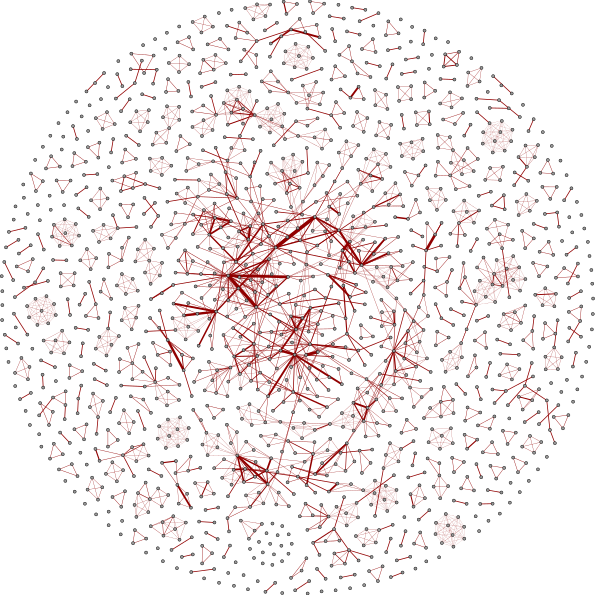
\includegraphics[width=\textwidth]{netscience}
\end{column}
\end{columns}
\end{frame}

\note{
A.-L. Barabasi, R. Albert, ``Emergence of scaling in random networks,'' Science, 286(5439):509–512 1999.\\
R. Albert, H. Jeong, A.-L. Barabsi, ``Error and attack tolerance of complex networks,'' Nature, 406(6794):378–382, 2000.\\
Data is from M.E.J. Newman, ``Finding community structure in networks using the eigenvectors of matrices'', Physical Review E 74, 036104 11 September 2006\prescite{newman2006}\\
Coauthorship of scientists working in network theory and experiment.
}

%%%%%%%%%%%%%%%%%%%%%%%%%%%%%%%%%%%%%%%%%

\begin{frame}
\frametitle{Network Effects}
Barab\'asi--Albert model of scale-free networks\prescite{barabasi1999, albert2000}.

Link-node power law distribution $P(k) \sim k^{-\gamma}$.
\begin{columns}[b]
\begin{column}[c]{0.5\textwidth}
\includegraphics[width=\textwidth]{powerlaw-netscience}
\end{column}
\begin{column}[c]{0.45\textwidth}
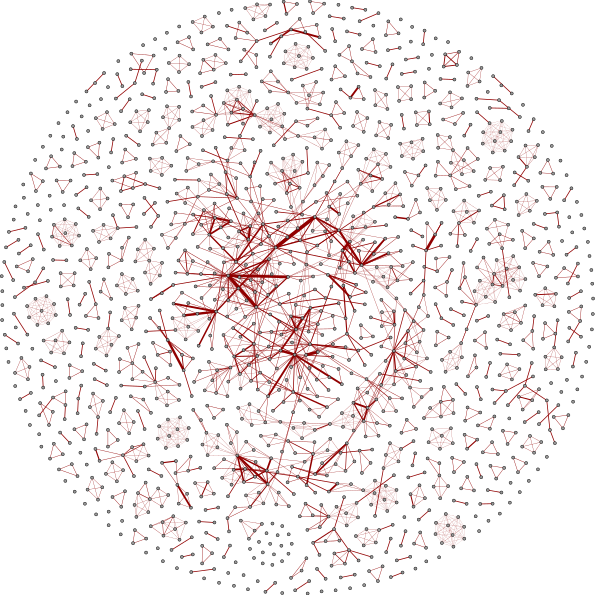
\includegraphics[width=\textwidth]{netscience}
\end{column}
\end{columns}
\end{frame}

%%%%%%%%%%%%%%%%%%%%%%%%%%%%%%%%%%%%%%%%%

\begin{frame}
\frametitle{Other topics covered}
\begin{enumerate}
\item Economics of vulnerabilities.
\begin{enumerate}
\item Vulnerability disclosure.
\item Certification.
\end{enumerate}
\item Economics of privacy.
\begin{enumerate}
\item Privacy gap between stated and revealed privacy.
\item How to measure value of privacy.
\end{enumerate}
\item Psychology.
\begin{enumerate}
\item Misperception of risk.
\item Phishing.
\end{enumerate}
\end{enumerate}
\end{frame}

%%%%%%%%%%%%%%%%%%%%%%%%%%%%%%%%%%%%%%%%%

\begin{frame}
\frametitle{Conclusion}
\begin{enumerate}
\item Security had been driven by technological approaches.
\item Understanding security required understanding economics and psychology.
\item Externalities prevented effective security actions.
\item Security decisions affected by incentives, asymmetric information, psychology.
\end{enumerate}


\end{frame}

%%%%%%%%%%%%%%%%%%%%%%%%%%%%%%%%%%%%%%%%%

\begin{frame}
\frametitle{Bibliography}
{\tiny
\bibliographystyle{apalike}
\bibliography{main}
}%
\end{frame}

%%%%%%%%%%%%%%%%%%%%%%%%%%%%%%%%%%%%%%%%%

\end{document}
